%conjunto de cadeias de 0's e 1's com número ímpar de 1‘s
\begin{center}

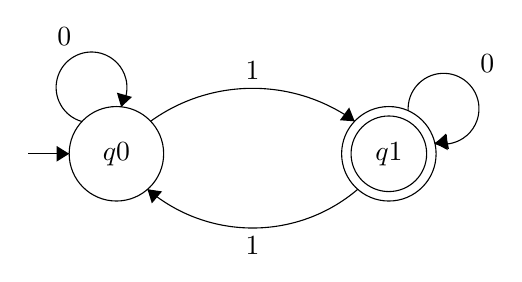
\begin{tikzpicture}[scale=0.2]
\tikzstyle{every node}+=[inner sep=0pt]
\draw [black] (28.1,-31.8) circle (3);
\draw (28.1,-31.8) node {$q0$};
\draw [black] (45.4,-31.8) circle (3);
\draw (45.4,-31.8) node {$q1$};
\draw [black] (45.4,-31.8) circle (2.4);
\draw [black] (43.432,-34.05) arc (-49.51444:-130.48556:10.292);
\fill [black] (30.07,-34.05) -- (30.35,-34.95) -- (31,-34.19);
\draw (36.75,-37.01) node [below] {$1$};
\draw [black] (30.266,-29.738) arc (125.83202:54.16798:11.076);
\fill [black] (43.23,-29.74) -- (42.88,-28.86) -- (42.29,-29.67);
\draw (36.75,-27.14) node [above] {$1$};
\draw [black] (48.7,-31.1) -- (48.33,-31.18);
\fill [black] (48.33,-31.18) -- (49.22,-31.5) -- (49.01,-30.52);
\draw [black] (46.628,-29.076) arc (183.47246:-104.52754:2.25);
\draw (51.17,-26.08) node [right] {$0$};
\fill [black] (48.31,-31.12) -- (49.14,-31.57) -- (49.08,-30.57);
\draw [black] (25.921,-29.755) arc (254.55605:-33.44395:2.25);
\draw (24.79,-24.96) node [above] {$0$};
\fill [black] (28.4,-28.83) -- (29.09,-28.19) -- (28.13,-27.92);
\draw [black] (22.5,-31.8) -- (25.1,-31.8);
\fill [black] (25.1,-31.8) -- (24.3,-31.3) -- (24.3,-32.3);
\end{tikzpicture}

\end{center}

